\documentclass[11pt,a4paper,titlepage]{ltjsarticle}
%
\usepackage{amsmath,amssymb}
\usepackage{bm}
\usepackage{physics}
\usepackage{graphicx}
\usepackage{ascmac}
\usepackage{cases}
\usepackage{here}
\usepackage{upgreek}
\usepackage{url}
\usepackage[backend=biber,sorting=none]{biblatex}
\addbibresource{cite.bib}
%
%
\title{2025年度 黒柳研究室\\SVM資料}
\author{古郷泰至}
\date{\today}
\begin{document}
\maketitle
%
%
\section{初めに}
SVMとはサポートベクターマシン(Support Vector Machine)の略であり,
分類問題や回帰問題に用いられる教師あり機械学習のアルゴリズムである.
SVMは最適化するパラメータが少なく高次元のデータや非線形なデータに対しても高い分類性能を発揮するが,
計算コストが高いためデータが大規模になると計算量が大きくなる\cite{masaya8028}.
また,SVMは主に2クラス分類で用いられるが多クラス分類にも拡張可能である.
本資料では,初めにSVMの理解に必要な知識であるラグランジュの未定乗数法,KKT条件,カーネル法について説明し
その後線形SVM,非線形SVMについて説明する.
\section{前提知識}
この章ではSVMを理解する上で必要となる知識について説明する.
\subsection{ラグランジュの未定乗数法}
ラグランジュの未定乗数法(Lagrange multiplier)とは等式制約のもとで多変数関数の最適化問題を解く手法である.\\
本資料では簡略化のため最適化する関数を2変数関数$f(x,y)$とし,$\bm{x} = [x,y]$とする.
式(\ref{equal})の等式制約のもとで関数$f(\bm{x})$が点$(a,b)$に極値を持つとする.
\begin{equation}
    \label{equal}
    g(x,y) = 0
\end{equation}
このとき,$\bm{x}$とラグランジュ乗数$\lambda$を変数に持つラグランジュ関数$L$を式(\ref{lagrange})のように定義する.
\begin{equation}
    \label{lagrange}
    L(\bm{x},\lambda) = f(\bm{x}) - \lambda g(\bm{x})
\end{equation}
このとき式(\ref{if})を満たす点では,式(\ref{then})を満たす$\lambda '$が存在する\cite{lagrange}.
\begin{equation}
    \label{if}
    \begin{aligned}
        \frac{\partial g}{\partial x}(a,b) \ne 0 \\
        または \\
        \frac{\partial g}{\partial y}(a,b) \ne 0
    \end{aligned}
\end{equation}
\begin{equation}
    \label{then}
    \begin{aligned}
        \frac{\partial L}{\partial x}(a,b,\lambda ') = 0\\
        \frac{\partial L}{\partial y}(a,b,\lambda ') = 0\\
        \frac{\partial L}{\partial \lambda}(a,b,\lambda ') = 0\\
    \end{aligned}
\end{equation}
式(\ref{then})の連立方程式を解くことで極値をとる点(a,b)を求められる.
この(a,b)を求める手法をラグランジュの未定乗数法という\cite{lagrange}.

\subsection{KKT条件}
KKT条件(Karush-Kuhn-Tucker conditions)とは,一般的な制約付き最適化問題の解が満たす条件である.
この制約は等式制約のみならずラグランジュの未定乗数法では扱えなかった不等式制約も含めた制約である.
KKT条件は目的としている最適化問題の最適性の必要十分条件であるため,この条件を満たす解は最適解であることが保証される.
式(\ref{inequ})のようなd次元のベクトル$\bm{x}$を変数とする複数の等式・不等式制約付き最適化問題を考える.
\begin{equation}
    \label{inequ}
    \begin{gathered}
        \underset{\bm{x}}{\min} f(\bm{x}) \\
        \text{s.t. } g_i(\bm{x}) \leq 0 \quad (i = 1,2\dots,G) \\
        h_j(\bm{x}) = 0 \quad (j = 1,2\dots,H)
    \end{gathered}
\end{equation}


このとき,ラグランジュ関数は以下の式(\ref{lag2})のように定義される.
\begin{equation}
    \label{lag2}
    \begin{gathered}
        L(\bm{x}, \bm{\lambda}, \bm{\mu}) = f(\bm{x}) + \sum_{i = 1}^{G}\lambda_i g_i(\bm{x}) + \sum_{j = 1}^{H} \mu_i h_i(\bm{x})\\
        ただし\\
        \bm{\lambda} = [\lambda_1,\lambda_2\dots\lambda_G]\\
        \bm{\mu} = [\mu_1,\mu_2\dots\mu_H]
    \end{gathered}
\end{equation}
ただし,不等式制約のラグランジュ未定乗数は$\lambda_i \geq 0$である.\\
この問題についての式(\ref{one})~(\ref{five})がKKT条件である.
データ$\bm{x}$に対して式(\ref{slater})を満たす点が少なくとも一つ存在するというスレーター条件を仮定した時にKKT条件を満たす$\lambda_i,\mu_i$が存在することが保証される.
このとき,KKT条件を満たすことが問題の最適解であるための必要十分条件となる.
式(\ref{one})はラグランジュ関数の微分条件,式(\ref{three})~(\ref{five})は等式・不等式制約とラグランジュ未定乗数の非負条件である.
また,式(\ref{two})は相補性条件と呼ばれ\cite{kkt-condition},この条件により最適解に関係のない不等式制約に対してラグランジュ未定乗数を0としている.
\begin{equation}
    \label{slater}
    g_i(\bm{x})<0,h_j(\bm{x})=0
\end{equation}
\begin{align}
        \frac{\partial }{\partial \bm{x}}L(\bm{x},\bm{\lambda},\bm{\mu}) = 0 \label{one}\\
        \lambda_i g_i(\bm{x}) = 0  (i = 1,2\dots G) \label{two}\\
        g_i(\bm{x}) \leq 0 (i = 1,2\dots G)\label{three}\\
        h_i(\bm{x}) = 0 (i = 1,2\dots H)\label{four}\\
        \lambda_i \geq 0 (i = 1,2\dots G)\label{five}
\end{align}
\clearpage

\subsection{カーネル法}
カーネル法とはもとの空間では線形分離不可能なデータ群をより高い次元数の空間(特徴空間)に写像することで線形分離可能にする手法のことである\cite{kerneltrick}.
このとき,写像する際の関数を$\phi(\bm{x})$とする.SVMにおいて最適化問題を解く上では$\phi(\bm{x})^\mathsf{T}\phi(\bm{x'})$のような内積の形でのみ現れるため,
内積の結果のみを返す新たな関数を考える.この関数をカーネル関数と呼び一般に式(\ref{karnel})のように表される.
カーネル関数を用いることによって$\phi(\bm{x})$を明示的に計算せずに内積を求めることができる.これをカーネルトリックという\cite{kerneltrick}.
\begin{equation}
    \label{karnel}
    K(\bm{x},\bm{x'}) = \phi(\bm{x})^\mathsf{T}\phi(\bm{x'})
\end{equation}
カーネル関数は式(\ref{taisyou})のような対称性と式(\ref{hansei})のような半正定値性を満たす必要がある\cite{ting}.
\begin{equation}
    \label{taisyou}
    K(\bm{x},\bm{x'}) = K(\bm{x'},\bm{x})
\end{equation}
\begin{equation}
    \label{hansei}
    \sum_{i=1}^{n}\sum_{j=1}^{n}c_ic_jK(\bm{x}_i,\bm{x}_j) \geq 0
\end{equation}
カーネル関数の具体例を表\ref{tab:kernels}に示す\cite{kernelchoice}.
利用するカーネル関数やそのハイパーパラメータによって得られる識別境界の様子が変化するため,データの特性に合わせてカーネル関数を選択する必要がある.
RBFカーネルの例では$\gamma$が大きいほど近い範囲のデータを特徴空間上で近い位置に写像するようになる.
\begin{table}[H]
    \centering
    \caption{カーネル関数の例}
    \label{tab:kernels}
    \begin{tabular}{|c|c|c|} \hline
        カーネル関数名 & 数式 & ハイパーパラメータ\\ \hline \hline
        線形カーネル & $K(\bm{x}, \bm{x}') = \bm{x}^\mathsf{T} \bm{x}'$ & 無し\\ \hline
        多項式カーネル & $K(\bm{x}, \bm{x}') = (\bm{x}^\mathsf{T} \bm{x}' + c)^q$ & c,q\\ \hline
        % ガウスカーネル & $K(\bm{x}, \bm{x}') = \exp\left(-\frac{\lVert \bm{x} - \bm{x}' \rVert^2}{2s^2}\right)$ & s\\ \hline
        シグモイドカーネル & $K(\bm{x}, \bm{x}') = \tanh(a\bm{x}^\mathsf{T} \bm{x}' + b)$ & a,b\\ \hline
        RBFカーネル & $K(\bm{x}, \bm{x}') = \exp\left(-\gamma \lVert \bm{x} - \bm{x}' \rVert^2\right)$ & \gamma\\ \hline
    \end{tabular}
\end{table}
\clearpage
カーネル関数のハイパーパラメータは事前に設定するため,SVMとは別に最適化する必要がある.
表\ref{tuning}にいくつかのハイパーパラメータの最適化手法を示す.
通常,パラメータは一度の操作では最適化されているか分からないため,選択されたパラメータを評価する手法が必要である.
評価にはしばしばデータをモデルの学習用のトレーニングデータとモデルの評価に使うテストデータに分けるクロスバリデーション(交差検証)が用いられる\cite{cross}.
ベイズ最適化はアルゴリズム内で獲得関数と呼ばれる関数を用いて次のパラメータを選択するため評価関数を用いない\cite{beiz}.

\begin{table}[H]
    \centering
    \caption{ハイパーパラメータ最適化の手法}
    \label{tuning}
    \begin{tabular}{|c|c|} \hline
        手法 & 説明 \\ \hline \hline
        グリッドサーチ & 事前に候補をそれぞれ複数用意し,それらの組み合わせをすべて試す手法\\ \hline
        ランダムサーチ & 候補をランダムに選択する操作を繰り返し行う手法 \\ \hline
        ベイズ最適化 & パラメータを確率的に探索する手法 \\ \hline
    \end{tabular}
\end{table}
\clearpage

\section{線形SVM}
\label{sec:linear}
線形SVMはd次元データの2クラス分類問題において式(\ref{bord})のような線形分類境界を導出するアルゴリズムである.

\begin{equation}
    \label{bord}
        f(\bm{x}) = \bm{\omega}^\mathsf{T}\bm{x} + \beta = 0 
\end{equation}
図\ref{fig:lin-sep},\ref{fig:nonlin-sep}のようなd次元のデータ群を考えたときにデータ群を分類するd-1次元の超平面を分離超平面と呼び,
分離超平面とその超平面に最も近いデータとの距離をマージンと呼ぶ.
また,分離超平面に最も近いデータのことをサポートベクトルと呼ぶ.
マージンには2つの種類があり,
図\ref{fig:lin-sep}のように線形分離可能(1つの直線で分けられる)なデータ群を前提としたマージンをハードマージン,
図\ref{fig:nonlin-sep}のように線形分離不可能(1つの直線で分けられない)なデータ群を前提としたマージンをソフトマージンと呼ぶ.
SVMはこのマージンを最大化するという考え方に基づいて分類境界を導出する.
\begin{figure}[H]
    \centering
    \begin{minipage}[b]{0.45\textwidth}
        \centering
        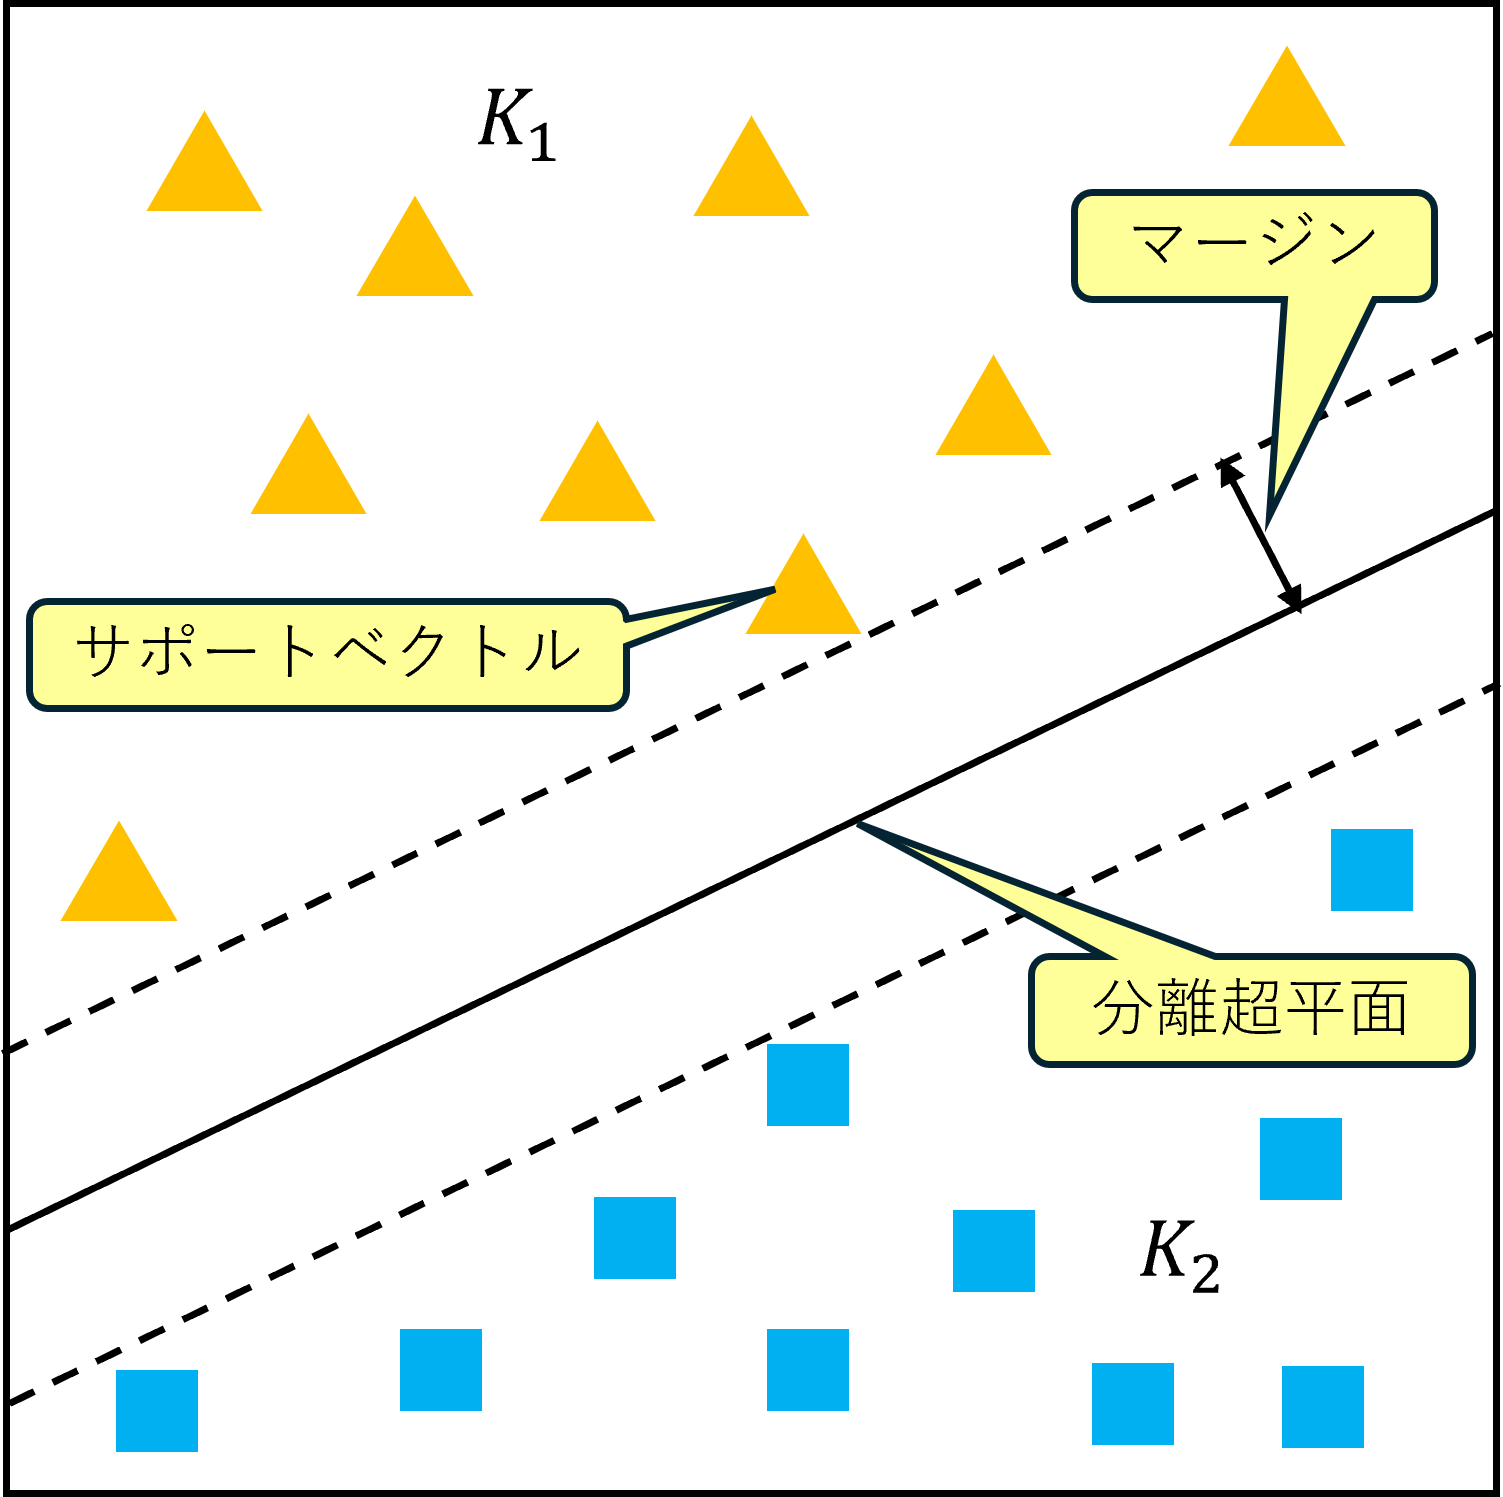
\includegraphics[width=1.0\columnwidth]{image/linear-separative.png}
        \caption{線形分離可能な問題の例}
        \label{fig:lin-sep}
    \end{minipage}
    \begin{minipage}[b]{0.45\textwidth}
        \centering
        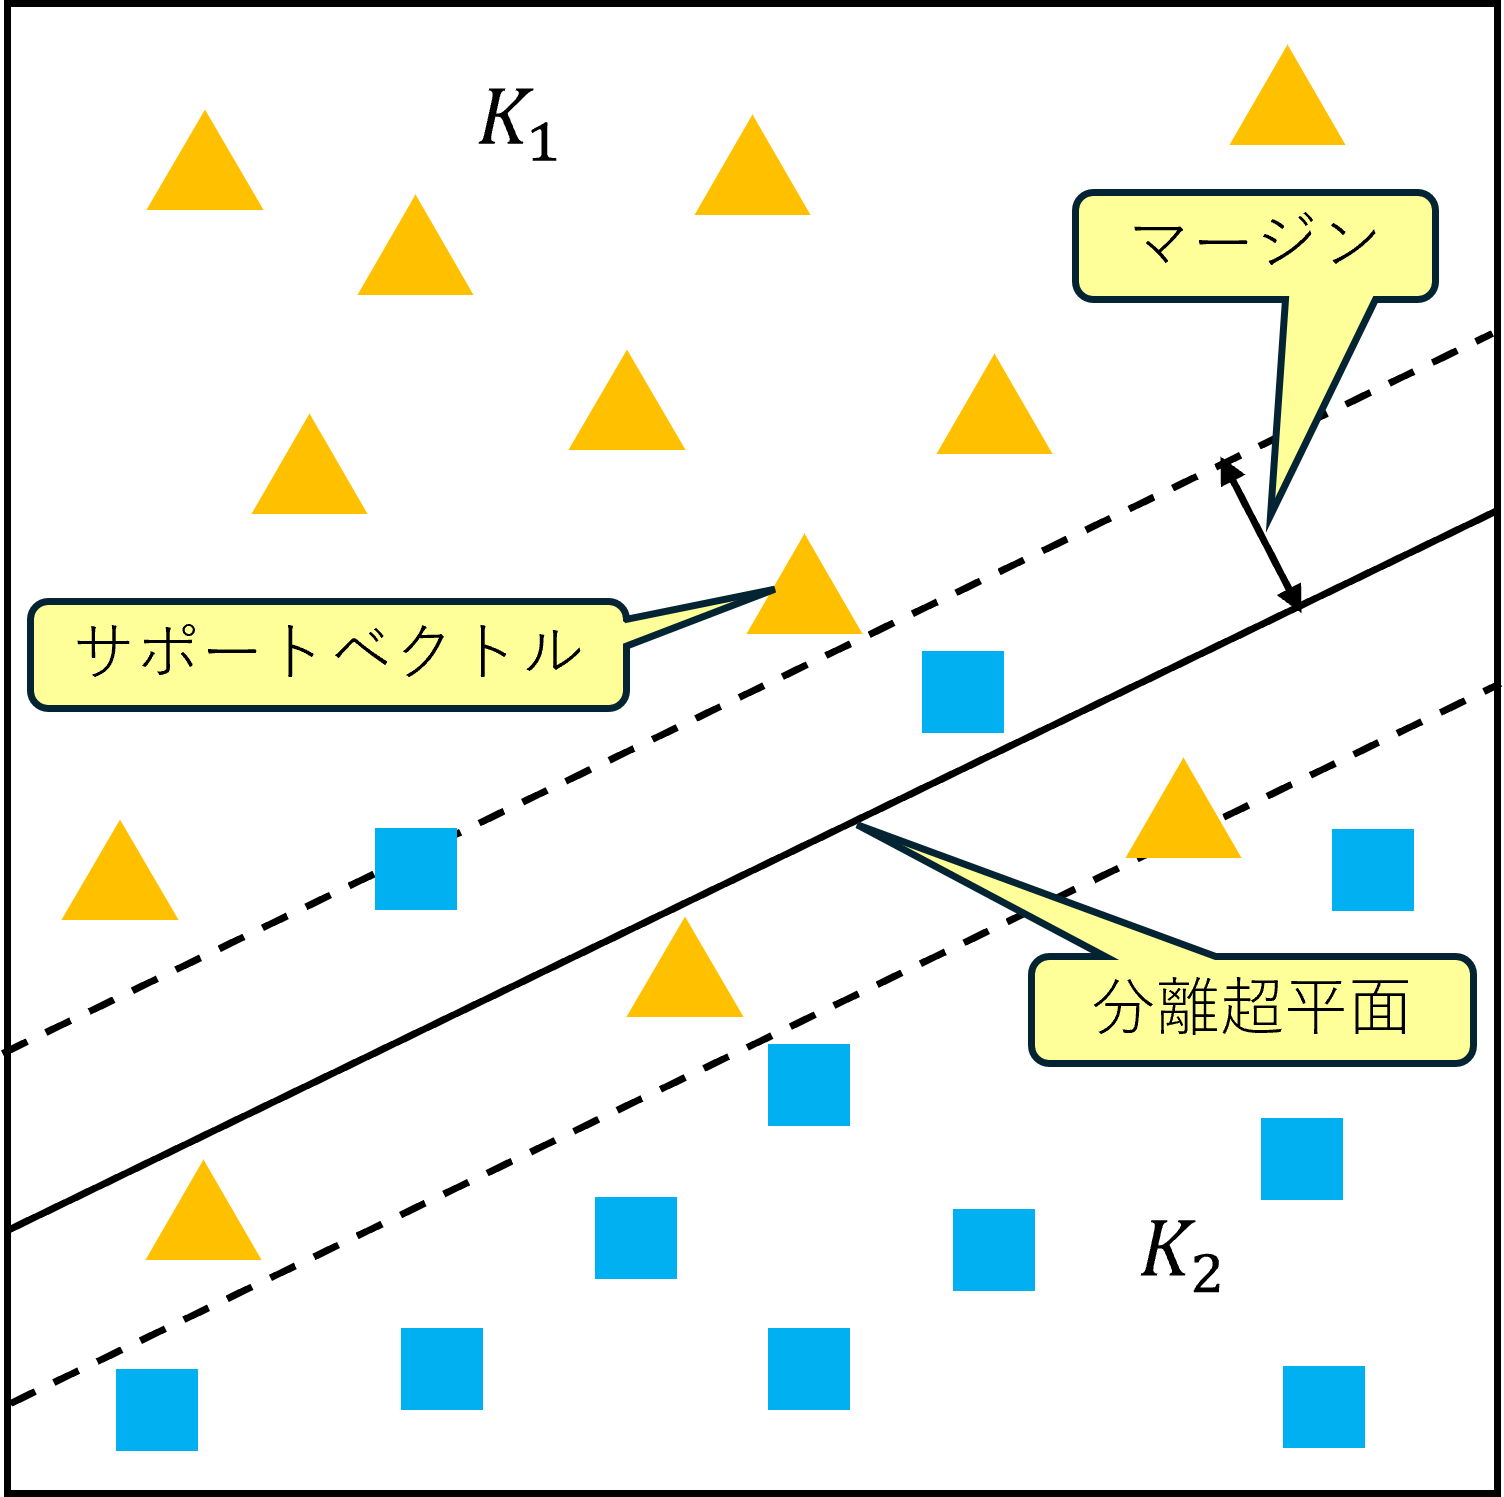
\includegraphics[width=1.0\columnwidth]{image/nonlinear-separative.png}
        \caption{線形分離不可能な問題の例}
        \label{fig:nonlin-sep}
    \end{minipage}
\end{figure}
図\ref{fig:lin-sep}では三角のデータをクラス$K_1$,四角のデータをクラス$K_2$に属すると考えると,式(\ref{bef})を満たす.
\begin{equation}
    \label{bef}
    \begin{split}
        \bm{\omega}^\mathsf{T}\bm{x}_i + \beta > 0\quad (\bm{x}_i \in K_1)\\
        \bm{\omega}^\mathsf{T}\bm{x}_i + \beta < 0\quad (\bm{x}_i \in K_2)
    \end{split}
\end{equation}
\clearpage
式(\ref{bef})をまとめるため,またSVMを設計するためにラベル変数$y_i$を式(\ref{class})で定義する.
このとき,すべてのデータ$\bm{x}_i$において式(\ref{class})を満たす超平面$f(\bm{x}) = 0$が存在するとき,線形分離可能という.
\begin{equation}
    \label{class}
    y_i =
    \begin{cases}
        +1 \quad(f(\bm{x}_i) > 0)\\
        -1 \quad(f(\bm{x}_i) < 0)
    \end{cases}
\end{equation}
式(\ref{class})を用いて式(\ref{bef})をまとめると式(\ref{success})のように表すことができる.
\begin{equation}
    \label{success}
    y_i(\bm{\omega}^\mathsf{T}\bm{x}_i + \beta) > 0\quad(i = 1,2 \dots N)
\end{equation}
\subsection{ハードマージンSVM}
\label{sec:hardmagin}
ハードマージンSVMは線形分離可能なデータを対象とした線形SVMである.
ある$\bm{x}_i$から識別境界までの距離$d_i$は式(\ref{distans})となる.
ただし$y_i$は式(\ref{class})で定義したラベル関数である.

\begin{equation}
    \label{distans}
    d_i = \frac{y_i(\bm{\omega}^\mathsf{T}\bm{x}_i + \beta)}{\begin{Vmatrix}\bm{\omega}\end{Vmatrix}}\quad(i = 1,2\dots n)
\end{equation}
今,線形分離可能なデータを仮定しているため,式(\ref{margin-con})をすべての$i$で満たす$\bm{\omega}$,
$\beta$及び$M$が存在するはずである.
\begin{equation}
    \label{margin-con}
    y_i(\bm{\omega}^\mathsf{T}\bm{x}_i + \beta) \geq M > 0
\end{equation}
このとき,マージンは式(\ref{distans}),(\ref{margin-con})とマージン最大化より式(\ref{margin})で求めることができる.
\begin{equation}
    \label{margin}
    \begin{gathered}
        \max_{\bm{\omega},\beta,M}\frac{M}{\begin{Vmatrix}\bm{\omega}\end{Vmatrix}}\\
        \text{s.t. } y_i(\bm{\omega}^\mathsf{T}\bm{x}_i + \beta) \geq M \quad (i=1,2\dots n)    
    \end{gathered}
\end{equation}
ここで式(\ref{redef})のように変数を定義しなおすと,式(\ref{margin})は式(\ref{new-margin})となる.
\begin{equation}
    \label{redef}
    \bm{\tilde{\omega}} = \frac{\bm{\omega}}{M},\tilde{\beta} = \frac{\beta}{M}
\end{equation}
\begin{equation}
    \label{new-margin}
    \begin{gathered}
        \max_{\bm{\tilde{\omega}},\tilde{\beta}}\frac{1}{\begin{Vmatrix}\bm{\tilde{\omega}}\end{Vmatrix}}\\
        \text{s.t. } y_i(\bm{\tilde{\omega}}^\mathsf{T}\bm{x}_i + \tilde{\beta}) \geq 1 \quad (i=1,2\dots n)
    \end{gathered}
\end{equation}
また,$\frac{1}{\begin{Vmatrix}\bm{\tilde{\omega}}\end{Vmatrix}}$の最大化は$\begin{Vmatrix}\bm{\tilde{\omega}}\end{Vmatrix}$の最小化と等価でありかつ,
$\begin{Vmatrix}\bm{\tilde{\omega}}\end{Vmatrix}$の最小化は$\begin{Vmatrix}\bm{\tilde{\omega}}\end{Vmatrix}^2$の最小化と等価なため,
式(\ref{new-margin})の変数を$\bm{\omega},\beta$に戻し変形することで,式(\ref{hardmargin})が得られる.ただし,後の計算のために$\frac{1}{2}$を加えている.
式(\ref{hardmargin})が線形分離可能な場合における最適化問題である.このような二次関数を一次式の制約のもと最適化する問題は二次計画問題と呼ばれる\cite{patern}.
\begin{equation}
    \label{hardmargin}
    \begin{gathered}
        \min_{\bm{\omega},\beta}\frac{1}{2}\begin{Vmatrix}\bm{\omega}\end{Vmatrix}^2\\
        \text{s.t. } y_i(\bm{\omega}^\mathsf{T}\bm{x}_i + \beta) \geq 1 \quad (i=1,2\dots n)
    \end{gathered}
\end{equation}
%Mは定数だし求めるのはパラメータだからそのままチルダを取ってもいい?的な感じ

\subsection{ソフトマージンSVM}
\label{sec:softmargin}
ソフトマージンSVMとは,線形分離不可能なデータを前提とし,誤判別を許容する線形SVMである.
ハードマージンSVMでは線形分離不可能な場合に式(\ref{hardmargin})の制約条件を満たす$\bm{\omega},\beta$が存在しない.
そこで,それぞれのデータについて$\xi_i \geq 0$だけ制約を違反しても良いこととする.このとき最適化問題は式(\ref{softmargin})となる.
ただし$\bm{\xi}=[\xi_1,\xi_2\dots\xi_n]$である.$\xi_i$はスラック変数と呼ばれ,制約違反の度合を表しているため小さい方が望ましい.
スラック変数の性質を図\ref{fig:slack},表\ref{tab:slack}に示す.
また,$C$は罰則の強さを調整するハイパーパラメータであり大きいほど過学習を起こしやすくなる\cite{Ckernel}.また,$C$が$\infty$のときハードマージンSVMに帰着する.
\begin{equation}
    \label{softmargin}
    \begin{gathered}
        \min_{\bm{\omega},\beta,\bm{\xi}}\frac{1}{2}\begin{Vmatrix}\bm{\omega}\end{Vmatrix}^2 + C\sum_{i=1}^{n}\xi_i\\
        \text{s.t. } \xi_i\geq0,C > 0, y_i(\bm{\omega}^\mathsf{T}\bm{x}_i + \beta) \geq 1-\xi_i \quad  (i = 1,2\dots n)
    \end{gathered}
\end{equation}
\begin{figure}[H]
    \centering
    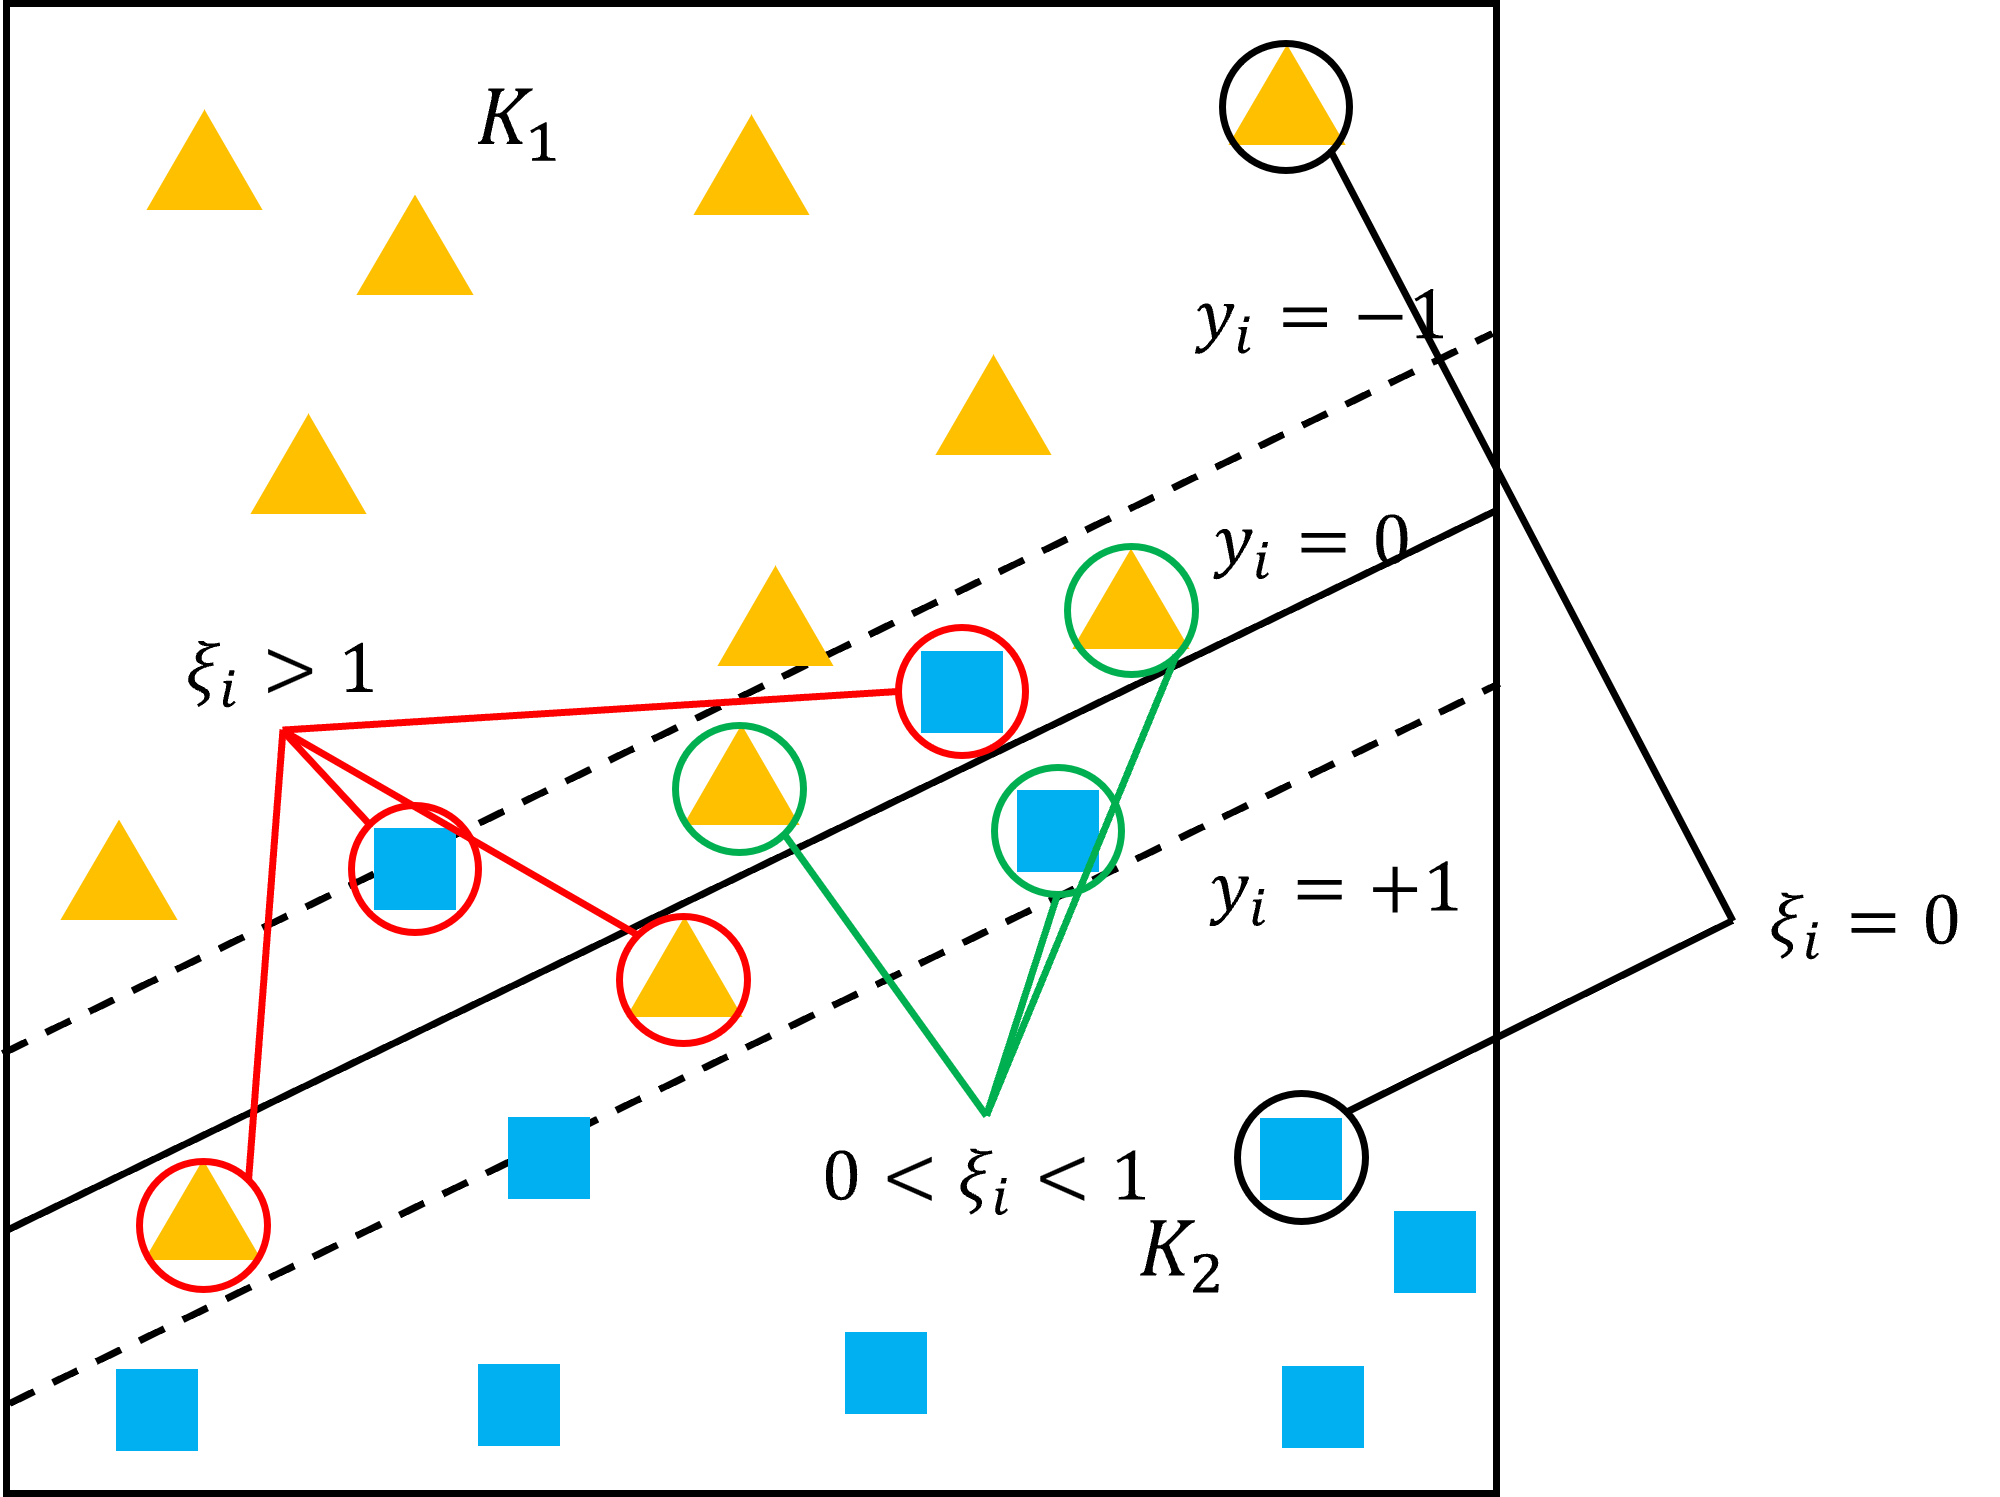
\includegraphics[width = 0.6\textwidth]{image/soft-mergin.png}
    \caption{スラック変数の例}
    \label{fig:slack}
\end{figure}
\begin{table}[H]
    \caption{スラック変数の性質}
    \begin{tabular}{|c|c|}\hline
        スラック変数 & データ点の位置\\ \hline
        $\xi_i = 0$ & 正しく分類されかつ,マージンの境界線上またはそれより外側に位置する.\\\hline
        $0 < \xi_i <1$ & 正しく分類されかつ,マージンの境界の内側で分類境界は越えていない \\ \hline
        $\xi_i > 1$ & 分類境界を越えており誤分類されている.\\\hline
    \end{tabular}
    \label{tab:slack}
\end{table}

\subsection{最適化問題の主問題と双対問題}
\label{sec:dual}
式(\ref{hardmargin}),式(\ref{softmargin})の最適化問題はSVMにおける主問題と呼ばれる.
これらの問題は単純に傾きを求める勾配法では制約条件を扱えず,扱うことのできる解法は低速であることが多い.
%勾配法は無制約最適化問題のアルゴリズム
そのため,SVMでは双対問題と呼ばれる主問題と等価な別の問題を解くことが多い.
双対問題とは,主問題に対して補集合となる,裏表の関係にある最適化問題である.
主問題と双対問題の間にはどちらか一方が最適解を持つなら,もう一方も最適解を持ち,主問題の最小値と双対問題の最大値が一致するという双対定理(dualibity theorem)が成立する.
そのためSVMでは双対問題を解くことによって最適化問題を簡単に解くことができる\cite{dual-problem}.

まず,ハードマージンSVMについての最適化問題である式(\ref{hardmargin})についてラグランジュの未定乗数法を用いると
ラグランジュ関数$L(\bm{x},\lambda)$は式(\ref{hardLag})となる.ただし$\bm{\lambda} = [\lambda_1,\lambda_2\dots\lambda_n]$である.
\begin{equation}
    \begin{gathered}
        \min_{\bm{\omega},\beta}\frac{1}{2}\begin{Vmatrix}\bm{\omega}\end{Vmatrix}^2\\
        \text{s.t. } y_i(\bm{\omega}^\mathsf{T}\bm{x}_i + \beta) \geq 1 \quad (i=1,2\dots n) \tag{\ref{hardmargin}}
    \end{gathered}
\end{equation}
\begin{equation}
    \label{hardLag}
    L(\bm{\omega},\beta,\bm{\lambda}) = \frac{1}{2}\begin{Vmatrix}\bm{\omega}\end{Vmatrix}^2 - \sum_{i=1}^{n}\lambda_i\{y_i(\bm{\omega}^\mathsf{T}\bm{x}_i + \beta) - 1\}
\end{equation}
このとき,ラグランジュ関数の微分条件より,式(\ref{con1})~(\ref{con3})の条件を満たす必要がある.
\begin{equation}
    \label{con1}
    \lambda_i \geq 0 \quad  (i =1,2\dots n)
\end{equation}
\begin{equation}
    \label{con2}
    \frac{\partial L}{\partial \bm{\omega}}(\bm{\omega},\beta,\bm{\lambda}) = \bm{\omega} - \sum_{i=1}^{n}\lambda_iy_i\bm{x}_i = 0
\end{equation}
\begin{equation}
    \label{con3}
    \frac{\partial L}{\partial \beta}(\bm{\omega},\beta,\bm{\lambda}) = -\sum_{i=1}^{n}\lambda_iy_i = 0    
\end{equation}
式(\ref{con2}),(\ref{con3})はそれぞれ変形すると,式(\ref{newcon2}),(\ref{newcon3})となる.
\begin{equation}
    \label{newcon2}
    \bm{\omega} = \sum_{i=1}^{n}\lambda_iy_i\bm{x}_i
\end{equation}
\begin{equation}
    \label{newcon3}
    \sum_{i=1}^{n}\lambda_iy_i = 0
\end{equation}
式(\ref{newcon2})を式(\ref{hardLag})に代入し整理すると,式(\ref{hard-dual})となる.
これにより,式(\ref{hardmargin})を最小化する$\bm{\omega},\beta$を求める主問題は,
双対問題は式(\ref{hard-dual})を最大化する$\bm{\lambda}$を求める問題に帰着することができる.
双対問題の制約条件は式(\ref{con1}),(\ref{newcon3})となる.
\begin{equation}
    \label{hard-dual}
    \max_{\bm{\lambda}}L(\bm{\omega},\beta,\bm{\lambda}) = \sum_{i=1}^{n}\lambda_i - \frac{1}{2}\sum_{i=1}^{n}\sum_{j=1}^{n}\lambda_i\lambda_jy_iy_j{\bm{x}_i}^\mathsf{T}\bm{x}_j
\end{equation}
\clearpage
同様にしてソフトマージンSVMの最適化問題である式(\ref{softmargin})について,ラグランジュ関数$L$は式(\ref{softLag})となる.
$\bm{\omega},\beta,\bm{\xi}$を主変数,$\bm{\lambda},\bm{\mu}$を双対変数といい$\bm{\lambda}\geq0,\bm{\mu}\geq0$である.
\begin{equation}
    \begin{gathered}
        \min_{\bm{\omega},\beta,\bm{\xi}}\frac{1}{2}\begin{Vmatrix}\bm{\omega}\end{Vmatrix}^2 + C\sum_{i=1}^{n}\xi_i\\
        \text{s.t. } \xi_i\geq0,C > 0, y_i(\bm{\omega}^\mathsf{T}\bm{x}_i + \beta) \geq 1-\xi_i \quad  (i = 1,2\dots n) \tag{\ref{softmargin}}
    \end{gathered}
\end{equation}
\begin{equation}
    \label{softLag}
    L(\bm{\omega},\beta,\bm{\xi},\bm{\lambda},\bm{\mu}) = \frac{1}{2}\begin{Vmatrix}\bm{\omega}\end{Vmatrix}^2 + C\sum_{i=1}^{n}\xi_i - \sum_{i=1}^{n}\lambda_i\{y_i(\bm{\omega}^\mathsf{T}\bm{x}_i + \beta) - 1+\xi_i\}-\sum_{i=1}^{n}\mu_i\xi_i
\end{equation}
このときのKKT条件は式(\ref{softcon1})~(\ref{softcon6})となる.
\begin{equation}
    \label{softcon1}
    \lambda_i\{1-\xi_i-y_i(\bm{\omega}^\mathsf{T}\bm{x}_i+\beta)\} = 0 
\end{equation}
\begin{equation}
    \label{softcon2}
    \mu_i\xi_i = 0
\end{equation}
\begin{equation}
    \label{softcon3}
    1-\xi_i-y_i(\bm{\omega}^\mathsf{T}\bm{x}_i+\beta) \leq 0
\end{equation}
\begin{equation}
    \label{softcon4}
    \xi_i \geq 0
\end{equation}
\begin{equation}
    \label{softcon5}
    \lambda_i\geq0
\end{equation}
\begin{equation}
    \label{softcon6}
    \mu_i\geq0
\end{equation}
式(\ref{softmargin})の双対問題は式(\ref{soft_dual})となる.
\begin{equation}
        \min_{\bm{\omega},\beta,\bm{\xi}}\frac{1}{2}\begin{Vmatrix}\bm{\omega}\end{Vmatrix}^2 + C\sum_{i=1}^{n}\xi_i \tag{\ref{softmargin}}
\end{equation}
\begin{equation}
    \label{soft_dual}
    \max_{\bm{\lambda},\bm{\mu}}\min_{\bm{\omega},\beta,\bm{\xi}}L(\bm{\omega},\beta,\bm{\xi},\bm{\lambda},\bm{\mu})
\end{equation}
このときハードマージンSVM同様にラグランジュ関数の微分条件より式(\ref{softLagcon1})~(\ref{softLagcon3})の条件を満たす必要がある.
%ここまで見た
\begin{equation}
    \label{softLagcon1}
    \frac{\partial L}{\partial \bm{\omega}} = \bm{\omega}-\sum_{i=1}^{n}\lambda_i y_i\bm{x}_i = 0
\end{equation}
\begin{equation}
    \label{softLagcon2}
    \frac{\partial L}{\partial \beta} = \sum_{i=1}^{n}\lambda_iy_i = 0
\end{equation}
\begin{equation}
    \label{softLagcon3}
    \frac{\partial L}{\partial \xi_i} = C - \lambda_i - \mu_i = 0
\end{equation}
式(\ref{softLag})を整理すると式(\ref{soft_Lag_1})となり,さらに式(\ref{softLagcon1})~(\ref{softLagcon3})を代入すると双対問題は
式(\ref{soft_dual2})となる.
\begin{equation}
    \label{soft_Lag_1}
    L(\bm{\omega},\beta,\bm{\xi},\bm{\lambda},\bm{\mu}) = \frac{1}{2}\begin{Vmatrix}\bm{\omega}\end{Vmatrix}^2  + \sum_{i=1}^{n}\lambda_i + \sum_{i=1}^{n}\lambda_iy_i(\bm{\omega}^\mathsf{T}\bm{x}_i + \beta)+\sum_{i=1}^{n}(C - \lambda_i - \mu_i)\xi_i
\end{equation}

\begin{equation}
    \label{soft_dual2}
    \begin{gathered}
        \max_{\bm{\lambda},\bm{\mu}}\min_{\bm{\omega},\beta,\bm{\xi}}-\frac{1}{2}\sum_{i=1}^{n}\sum_{j=1}^{n}\lambda_i\lambda_j y_i y_j \bm{x}_i^\mathsf{T}\bm{x}_j+\sum_{i=1}^{n}\lambda_i\\
    \end{gathered}
\end{equation}

このときの制約条件は双対変数$\bm{\lambda},\bm{\mu}$が非負であることと式(\ref{softLagcon2}),(\ref{softLagcon3})より式(\ref{soft_dual_con})となる.
\begin{equation}
    \label{soft_dual_con}
    \begin{gathered}
        0\leq \lambda_i \leq C\\
        \sum_{i=1}^{n}\lambda_iy_i = 0
    \end{gathered}
\end{equation}

\subsection{線形分類境界の導出}
\label{sec:dousyutsu}
この章では,式(\ref{bord})で表される線形分類境界を求める手法について説明する.
\begin{equation}
    f(\bm{x}) = \bm{\omega}^\mathsf{T}\bm{x} + \beta = 0 \tag{\ref{bord}}
\end{equation}
\ref{sec:dual}節では主問題を双対変数$\lambda_i$のみの関数についての双対問題に帰着させたが,
ここで$\lambda_i$の性質について表\ref{tab:lambda}に示す.この性質から,
$0<\lambda_i\leq C$であるデータのみが境界に関係することが分かる.
\begin{table}[H]
    \centering
    \caption{双対変数の性質}
    \label{tab:lambda}
    \begin{tabular}{|c|c|c|}\hline
        データの位置 & $\lambda_i$ & 分類境界の決定への影響 \\ \hline \hline
        \begin{tabular}{c}
            マージンの外側 \\
            $(y_i(\bm{\omega}^\mathsf{T}\bm{x}_i + \beta) > 1)$
        \end{tabular} & $\lambda_i = 0$ & 無し\\ \hline
        \begin{tabular}{c}
            マージン上\\
            $(y_i(\bm{\omega}^\mathsf{T}\bm{x}_i + \beta) = 1)$
        \end{tabular} & $0 < \lambda_i < C$ & 有り\\ \hline
        \begin{tabular}{c}
            マージンの内側\\
            $(y_i(\bm{\omega}^\mathsf{T}\bm{x}_i + \beta) < 1)$
        \end{tabular} & $\lambda_i = C$ & 有り\\ \hline
        
    \end{tabular}
\end{table}
ここで分類境界の式(\ref{bord})の$\bm{\omega}$に式(\ref{newcon2})を代入すると式(\ref{newbord})となる.
$\bm{\omega}$及び$f(\bm{x})$は$\lambda_i,y_i,\bm{x}_i$の積の線形結合により表されている.
また,総和を取る項数はデータ数に等しいため,全データを参照して分類境界を決定していることが分かる.
\begin{equation}
    \label{newbord}
    f(\bm{x}) = \sum_{i=1}^{n}\lambda_iy_i\bm{x}_i^\mathsf{T}\bm{x} + \beta
\end{equation}
また,$\beta$に関して別の表現を考える.KKT条件のうち相補性条件の式(\ref{softcon2})から
ラグランジュ関数の微分条件式(\ref{softLagcon3})により$\mu_i$を消去したものを
式(\ref{mudelete1})に示す.
\begin{equation}
    \mu_i\xi_i = 0 \tag{\ref{softcon2}}
\end{equation}
\begin{equation}
    \frac{\partial L}{\partial \xi_i} = C - \lambda_i - \mu_i = 0 \tag{\ref{softLagcon3}}
\end{equation}
\begin{equation}
    \label{mudelete1}
    (C-\lambda_i)\xi_i = 0
\end{equation}
表\ref{tab:lambda}より分類境界の決定に関係するのは$0<\lambda_i\leq C$のときであり,
$0<\lambda_i < C$条件下では$\lambda_i\neq0,C-\lambda_i \neq0$が成立するので,
式(\ref{softcon1}),(\ref{mudelete1})より式(\ref{mudelete2}),(\ref{mudelete3})が成り立つ.
\begin{equation}
    \lambda_i\{1-\xi_i-y_i(\bm{\omega}^\mathsf{T}\bm{x}_i+\beta)\} = 0  \tag{\ref{softcon1}}
\end{equation}
\begin{equation}
    \label{mudelete2}
    1-\xi_i-y_i(\bm{\omega}^\mathsf{T}\bm{x}_i+\beta) = 0 
\end{equation}
\begin{equation}
    \label{mudelete3}
    \xi_i = 0
\end{equation}
式(\ref{mudelete2}),(\ref{mudelete3})をまとめ,式(\ref{newcon2})により$\bm{\omega}$を消去すると式(\ref{omegadelete})となる.
\begin{equation}
    \label{omegadelete}
    y_i\left(\sum_{j=1}^{n}\lambda_jy_j\bm{x}_j^\mathsf{T}\bm{x}_i + \beta\right) = 1
\end{equation}
$y_i$は$1$または$-1$のどちらかなので$y_i^2=1$である.式(\ref{omegadelete})の両辺に$y_i$をかけて$\beta$について整理すると,
式(\ref{beta})となる.
\begin{equation}
    \label{beta}
    \beta = y_i - \sum_{j=1}^{n}\lambda_jy_j\bm{x}_j^\mathsf{T}\bm{x}_i
\end{equation}
したがって,あるサポートベクトル$\bm{x}_i$により$\beta$を導くことができる.しかしサポートベクトルは複数存在し得るため,
式(\ref{support})のように複数のサポートベクトルについて求めた$\beta$の平均を計算することで誤差を小さくすることができる.
ただし$SV$はサポートベクトルのインデックスの集合で$|SV|$はインデックスの個数である.
\begin{equation}
    \label{support}
    \beta = \frac{1}{|SV|}\sum_{i\in SV}\left(y_i - \sum_{j=1}^{n}\lambda_jy_j\bm{x}_j^\mathsf{T}\bm{x}_i\right)
\end{equation}
式(\ref{support})により$\beta$を求められるが,サポートベクトル以外のデータでは$\lambda_i = 0$であり,分類境界の決定に影響しない.
このようにデータのうち一部の少ない要素が本質的な情報を持つ性質をスパース性と呼び\cite{sparce},スパース性のあるデータにおいて$\lambda_i = 0$となる
データの計算は省略することができる.スパース性を踏まえた上で式(\ref{support})を書き直すと式(\ref{support2})となり,計算量を減らすことができる.
\begin{equation}
    \label{support2}
    \beta = \frac{1}{|SV|}\sum_{i \in SV}\left(y_i - \sum_{j \in SV}\lambda_jy_j\bm{x}_j^\mathsf{T}\bm{x}_i\right)
\end{equation}

\section{非線形SVM}
線形分離不可能なデータに対してソフトマージンSVMを説明したが,本章では線形分離不可能なデータに対する非線形SVMについて説明する.
特に今回は線形分離不可能なデータを線形分離可能なデータとなるように
元のデータ空間から別のデータ空間に射影する,カーネルSVMについて説明する.
図\ref{fig:nonlin-karnel}のような元のデータ空間からの射影先の空間を特徴空間という.
\begin{figure}[H]
    \centering
    \centering
    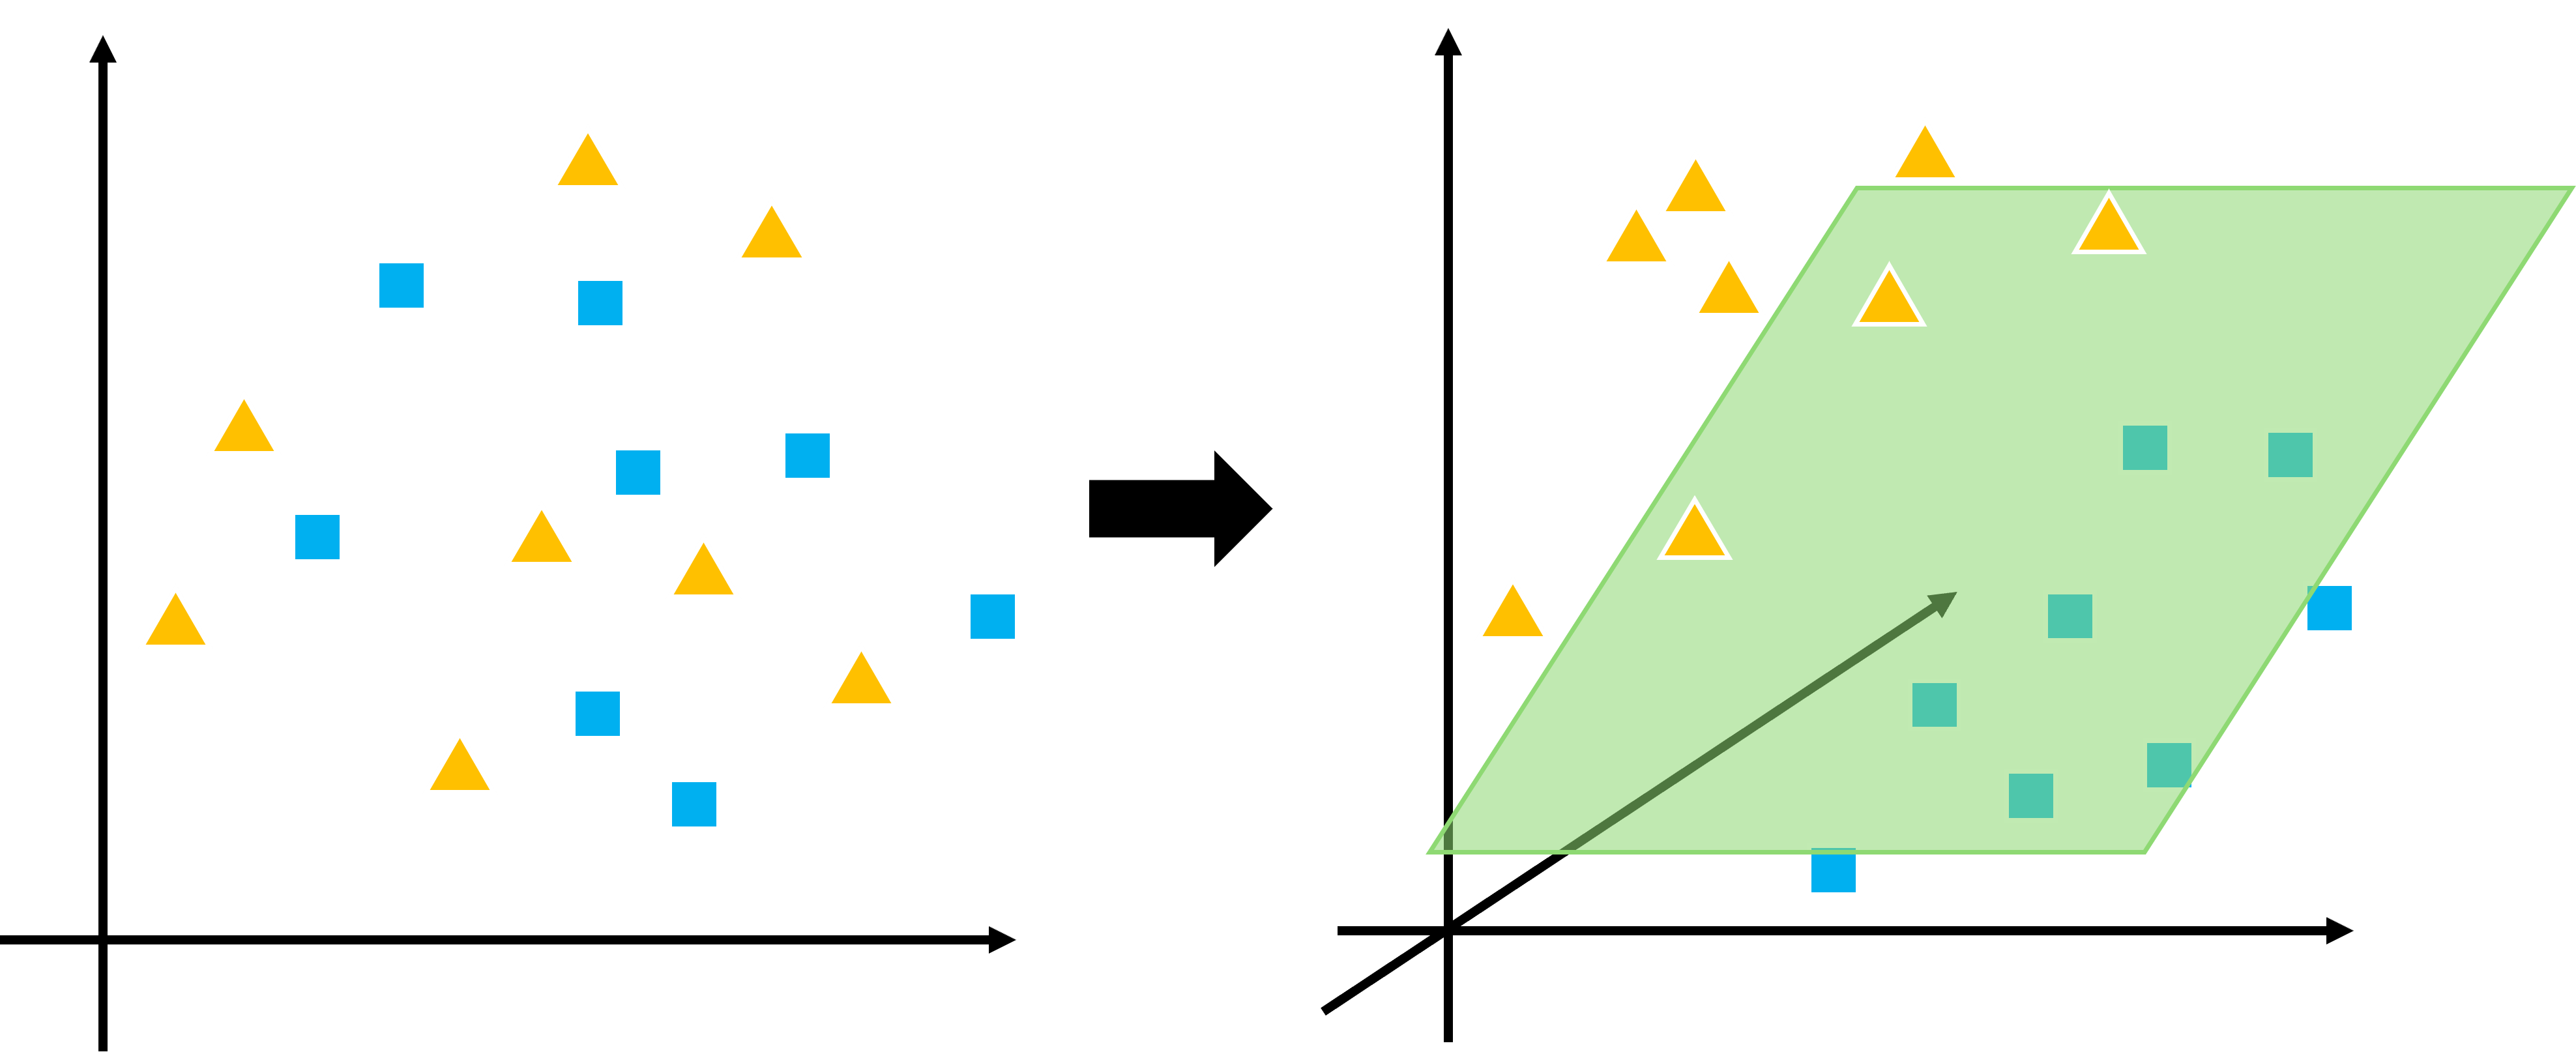
\includegraphics[width=0.9\textwidth]{image/karnel.png}
    \caption{特徴空間への写像}
    \label{fig:nonlin-karnel}
\end{figure}

データ$\bm{x}$を射影した$\phi(\bm{x})$の空間で考えた時,$\phi(\bm{x}) = \bm{x}$とすれば線形SVMに帰着する.
したがって,分類境界の式(\ref{bord})を書き換えると,式(\ref{nonlinbord})となる.
\begin{equation}
    \label{nonlinbord}
    f(\bm{x}) = \bm{\omega}^\mathsf{T}\phi(\bm{x})+\beta
\end{equation}
式(\ref{nonlinbord})に対する最適化問題は\ref{sec:dual}節で説明した導出方法を用いることができるため,双対問題は式(\ref{nonlindual})のように表すことができる.
\begin{equation}
    \label{nonlindual}
    \begin{gathered}
        \max_{\bm{\lambda}}\left(\sum_{i=1}^{n}\lambda_i-\frac{1}{2}\sum_{i=1}^{n}\sum_{j=1}^{n}\lambda_i\lambda_jy_iy_j\phi(\bm{x}_i)^\mathsf{T}\phi(\bm{x}_j)\right)\\
        \text{s.t. }\sum_{i=1}^{n}\lambda_iy_i=0,0\leq\lambda_i\leq C
    \end{gathered}
\end{equation}
ここで$\phi(\bm{x}_i)^\mathsf{T}\phi(\bm{x}_j)$は内積であるため,カーネル関数$K$を用いると式(\ref{nonlinkarnel})と書き換えられる.
\begin{equation}
    \label{nonlinkarnel}
    \begin{gathered}
        \max_{\bm{\lambda}}\left(\sum_{i=1}^{n}\lambda_i-\frac{1}{2}\sum_{i=1}^{n}\sum_{j=1}^{n}\lambda_i\lambda_jy_iy_jK(\bm{x}_i,\bm{x}_j)\right)\\
        \text{s.t. }\sum_{i=1}^{n}\lambda_iy_i=0,0\leq\lambda_i\leq C
    \end{gathered}
\end{equation}
また,線形SVMにおいて分類境界は式(\ref{newbord})のように書けるため非線形SVMも同様に
式(\ref{newnonlinbord})となり,この式にカーネル関数を用いると式(\ref{NewNonLinBordKarnel})と書ける.
\begin{equation}
    f(\bm{x}) = \sum_{i=1}^{n}\lambda_iy_i\bm{x}_i^\mathsf{T}\bm{x} + \beta \tag{\ref{newbord}}
\end{equation}
\begin{equation}
    \label{newnonlinbord}
    f(\bm{x}) = \sum_{i=1}^{n}\lambda_iy_i\phi(\bm{x}_i)^\mathsf{T}\phi(\bm{x}) + \beta
\end{equation}
\begin{equation}
    \label{NewNonLinBordKarnel}
    f(\bm{x}) = \sum_{i=1}^{n}\lambda_iy_iK(\bm{x},\bm{x}_i) + \beta
\end{equation}
さらに,\ref{sec:dousyutsu}節と同様に考えて$\beta$は式(\ref{nonlinbeta})で推定される.
\begin{equation}
    \label{nonlinbeta}
    \beta = \frac{1}{|SV|}\sum_{i \in SV}\left(y_i - \sum_{i \in SV}\lambda_jy_jK(\bm{x}_i,\bm{x}_j)\right)
\end{equation}

\section{最適化問題を解くアルゴリズム}
ここまでの章では求めるべき最適化問題の導出方法を説明したが,本章では求めた最適化問題の解となる$\lambda_i$を求めるアルゴリズムについて説明する.
\subsection{最急降下法}
\label{saikyuu}
図\ref{parabora}のようにある点から最も傾きが急な方向に点を少し動かし,動かした点でまた傾きが急な方向に点を動かすという操作を繰り返すことで局所解を見つける方法を最急降下法という\cite{gradient-descent}.
\begin{figure}[H]
    \centering
    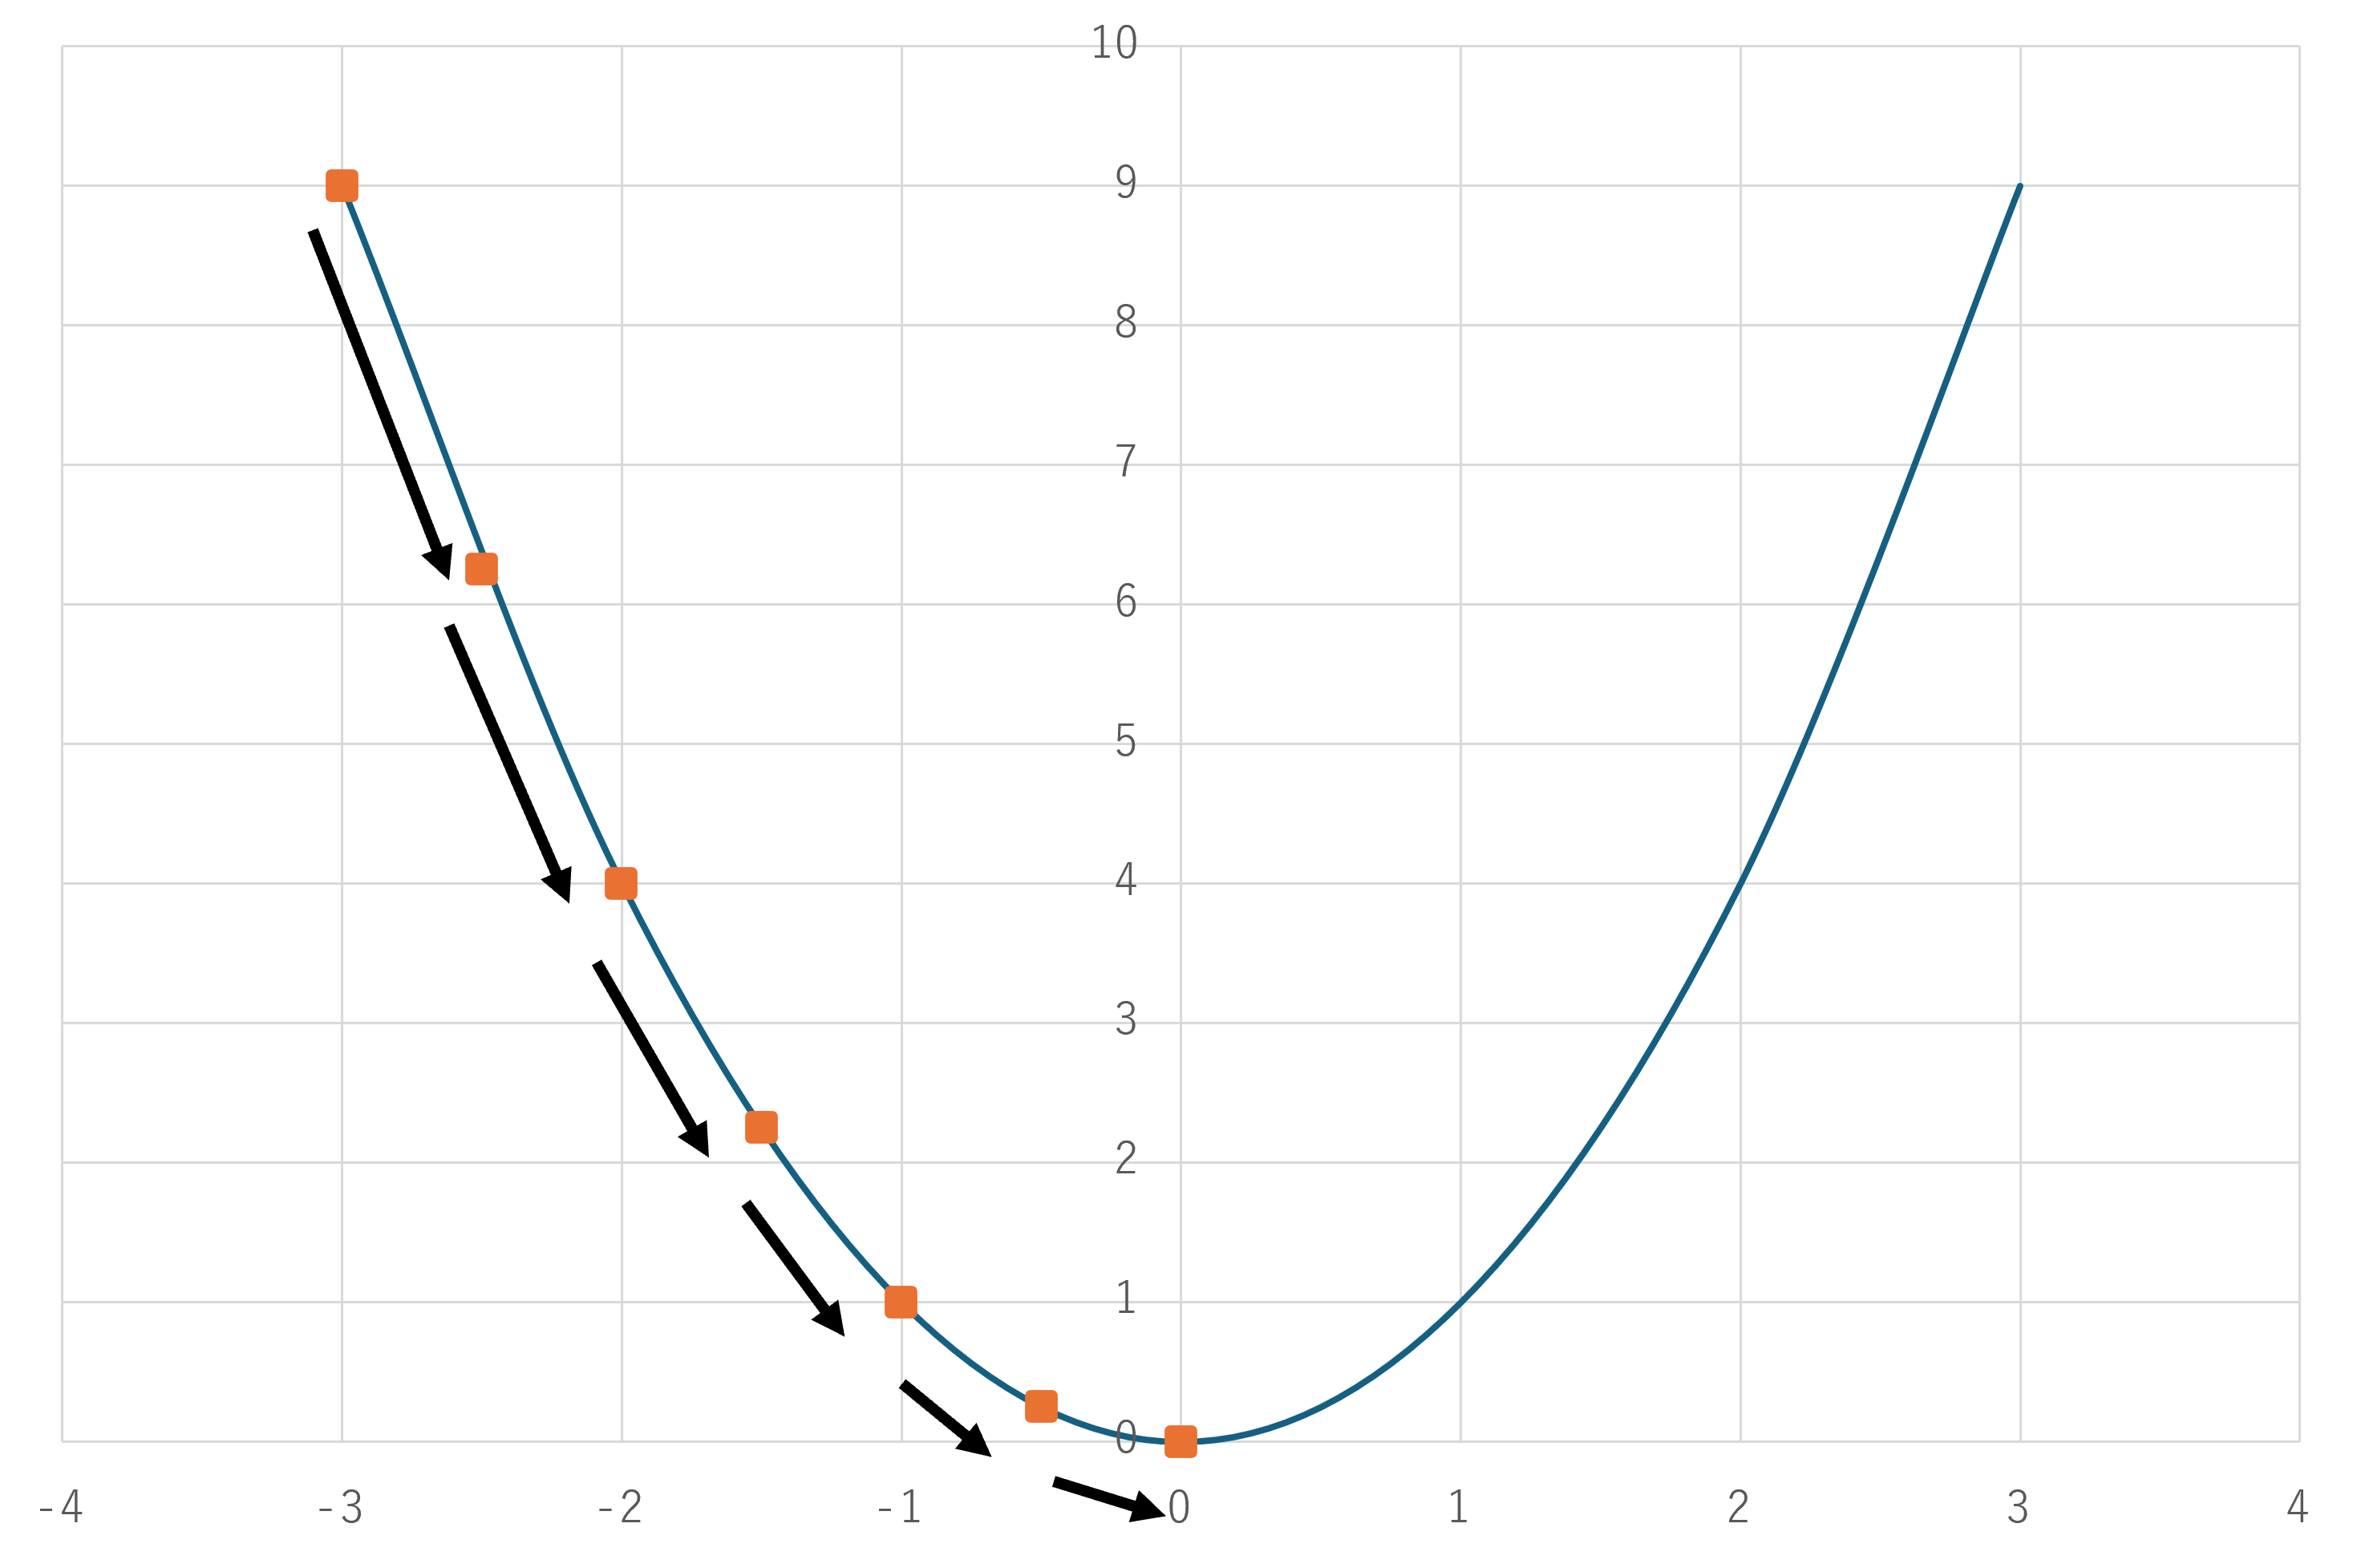
\includegraphics[width = 0.8\textwidth]{image/houbutsu.png}
    \caption{最急降下法}
    \label{parabora}
\end{figure}
最急降下法を用いて$\lambda_i$を求める.式(\ref{nonlinkarnel})の
$$\sum_{i=1}^{n}\lambda_i-\frac{1}{2}\sum_{i=1}^{n}\sum_{j=1}^{n}\lambda_i\lambda_jy_iy_jK(\bm{x}_i,\bm{x}_j)$$
の部分を$L(\bm{\lambda})$としこの関数を最大化する$\bm{\lambda}$を求めることを考える.
今回は最大化する$\bm{\lambda}$を求めるため,$L(\bm{\lambda})$が増加する方向,即ち勾配ベクトルの方向に$\bm{\lambda}$を更新する.
更新する際の更新規則は式(\ref{renewbeta})となる.ただし$\lambda_i^{(k)}$は$k$回目の更新時の$\lambda_i$である.また,初期値である$\lambda_i^{(0)}$には適当な値が設定されているものとする.(多くの場合で$\lambda_i$ = 0)
また,$\tau$は学習率と呼ばれる$0<\tau\leq1$の値を取るハイパーパラメータである.この学習率は別の分野ではステップ幅とも呼ばれ,更新時にどれだけ大きく$\lambda_i$を変化させるかを決める.
大きすぎると発散してしまい学習が進まず,小さすぎると収束するのに必要な更新回数が増える.そのため適切な学習率を設定する必要がある.式(\ref{renewbeta})によりすべての$\lambda_i$を求めることができる.
\begin{equation}
    \label{renewbeta}
    \begin{gathered}
        \lambda_i^{(k+1)} = \lambda_i^{(k)}+\tau\frac{\partial L(\bm{\lambda})}{\partial \lambda_i}\\
        =\lambda_i^{(k)} + \tau \left\{1 - \sum_{j=1}^{n}\lambda_i^{(k)}y_iy_jK(\bm{x}_i,\bm{x}_j)\right\}
    \end{gathered}
\end{equation}

\subsection{SMO}
\label{smo}
最急降下法では1変数ずつ更新したが,双対問題でこの方法を使うと式(\ref{nonlinkarnel})の制約条件を満たさなくなってしまう.
そこで,2変数ずつ更新することで制約条件を満たしながら最適化する.SVMにおいてこの手法をSMO(Sequential Minimal Optimization)と呼ぶ\cite{optimize}.
まず,表記の簡単のため$\alpha_i = y_i\lambda_i$,$k_{ij} = K(\bm{x}_i,\bm{x}_j)$とすると,式(\ref{nonlinkarnel})は式(\ref{newnonlinkarnel})と書ける.
\begin{equation}
    \label{newnonlinkarnel}
    \begin{gathered}
        \max_{\bm{\alpha}} -\frac{1}{2}\sum_{i=1}^{n}\sum_{j=1}^{n}\alpha_i\alpha_jk_{ij} + \sum_{i=1}^{n}y_i\alpha_i\\
        \text{s.t }0\leq\alpha_i\leq C \quad ( y_i = +1)\\
        -C \leq \alpha_i \leq 0 \quad ( y_i = -1)\\
        \sum_{i=1}^{n}\alpha_i = 0
    \end{gathered}
\end{equation}
ここで二つの変数$\alpha_h$と$\alpha_k$を更新することを考える.このとき更新量を$\Delta\alpha_h$とすると式(\ref{step})のようにすることで制約条件を満たしながら更新することができる.
\begin{equation}
    \label{step}
    \begin{gathered}
        \alpha_h^{(k+1)} = \alpha_h^{(k)} + \Delta\alpha_h\\
        \alpha_k^{(k+1)} = \alpha_k^{(k)} - \Delta\alpha_h
    \end{gathered}
\end{equation}
次に,更新後の$\alpha_h^{(k+1)}$と$\alpha_k^{(k+1)}$も式(\ref{paramscon})のように式(\ref{nonlinkarnel})の一つ目と二つ目の制約を満たす必要があるため,
$\Delta\alpha_h$にも制約を加える必要がある.
\begin{equation}
    \label{paramscon}
    \begin{gathered}
        0\leq\alpha_i + \Delta\alpha_h \leq C\quad(i \in {i | y_i = +1})\\
        -C \leq \alpha_i + \Delta\alpha_h \leq 0 \quad (i \in {i | y_i = -1})
    \end{gathered}
\end{equation}
これを$y_h$,$y_k$の符号のそれぞれの組み合わせに対して考えると,$\Delta\alpha_h$は式(\ref{deltacon})を満たす必要がある.
\begin{equation}
    \label{deltacon}
    \begin{gathered}
        \max(-\alpha_h,\alpha_k-C) \leq \Delta\alpha_h \leq \min(C-\alpha_h,\alpha_k)\quad(y_h=+1,y_k=+1)\\
        \max(-\alpha_h,\alpha_k) \leq \Delta\alpha_h \leq \min(C-\alpha_h,C+\alpha_k)\quad(y_h=+1,y_k=-1)\\
        \max(-C-\alpha_h,\alpha_k-C) \leq \Delta\alpha_h \leq \min(-\alpha_h,\alpha_k)\quad(y_h=-1,y_k=+1)\\
        \max(-C-\alpha_h,\alpha_k) \leq \Delta\alpha_h \leq \min(-\alpha_h,C+ \alpha_k)\quad(y_h=-1,y_k=-1)
    \end{gathered}
\end{equation}
式(\ref{newnonlinkarnel})に式(\ref{step})を代入して$\Delta\alpha_h$についての制約付き最適化問題として表すと式(\ref{nonlindelta})となる.
ただし,$L$,$U$は式(\ref{deltacon})の4つの不等式のうちのいずれかであり$C'$は定数項である.
\begin{equation}
    \label{nonlindelta}
    \begin{gathered}
        \max_{\bm{\alpha}}\frac{1}{2}(-k_{hh} + 2k_{hk} - k_{kk})\Delta\alpha_h^2+\left(y_h-\sum_{i\in n}\alpha_ik_{ih} - y_k + \sum_{i \in n}\alpha_ik_{ik}\right)\Delta\alpha_h + C'\\
        \text{s.t. } L \leq \Delta\alpha_h \leq U
    \end{gathered}
\end{equation}
式(\ref{nonlindelta})は変数が$\Delta\alpha_h$1つの制約付き2次関数の最小化問題となるので,$\Delta\alpha_h$は式(\ref{deltaans})となる.
これを用いることで$\lambda_i$を求めることができる.
\begin{equation}
    \label{deltaans}
    \Delta\alpha_h =
    \begin{cases}
        \displaystyle L & \text{if } L > \Delta\alpha_h \\
        \displaystyle U & \text{if } U < \Delta\alpha_h \\
        \displaystyle \frac{-y_h + y_k + \sum_{i\in n}\alpha_i(k_{ih} - k_{ik})}{-k_{hh} + 2k_{hk} - k_{kk}} & \text{otherwise}
    \end{cases}
\end{equation}


\section{まとめ}
最後に,ハードマージン線形SVMによる分類境界の求め方をまとめたものを図\ref{flow}に示す\cite{soft-mergin}.この図のようにして分類問題を解くことができる.
\begin{figure}[H]
    \centering
    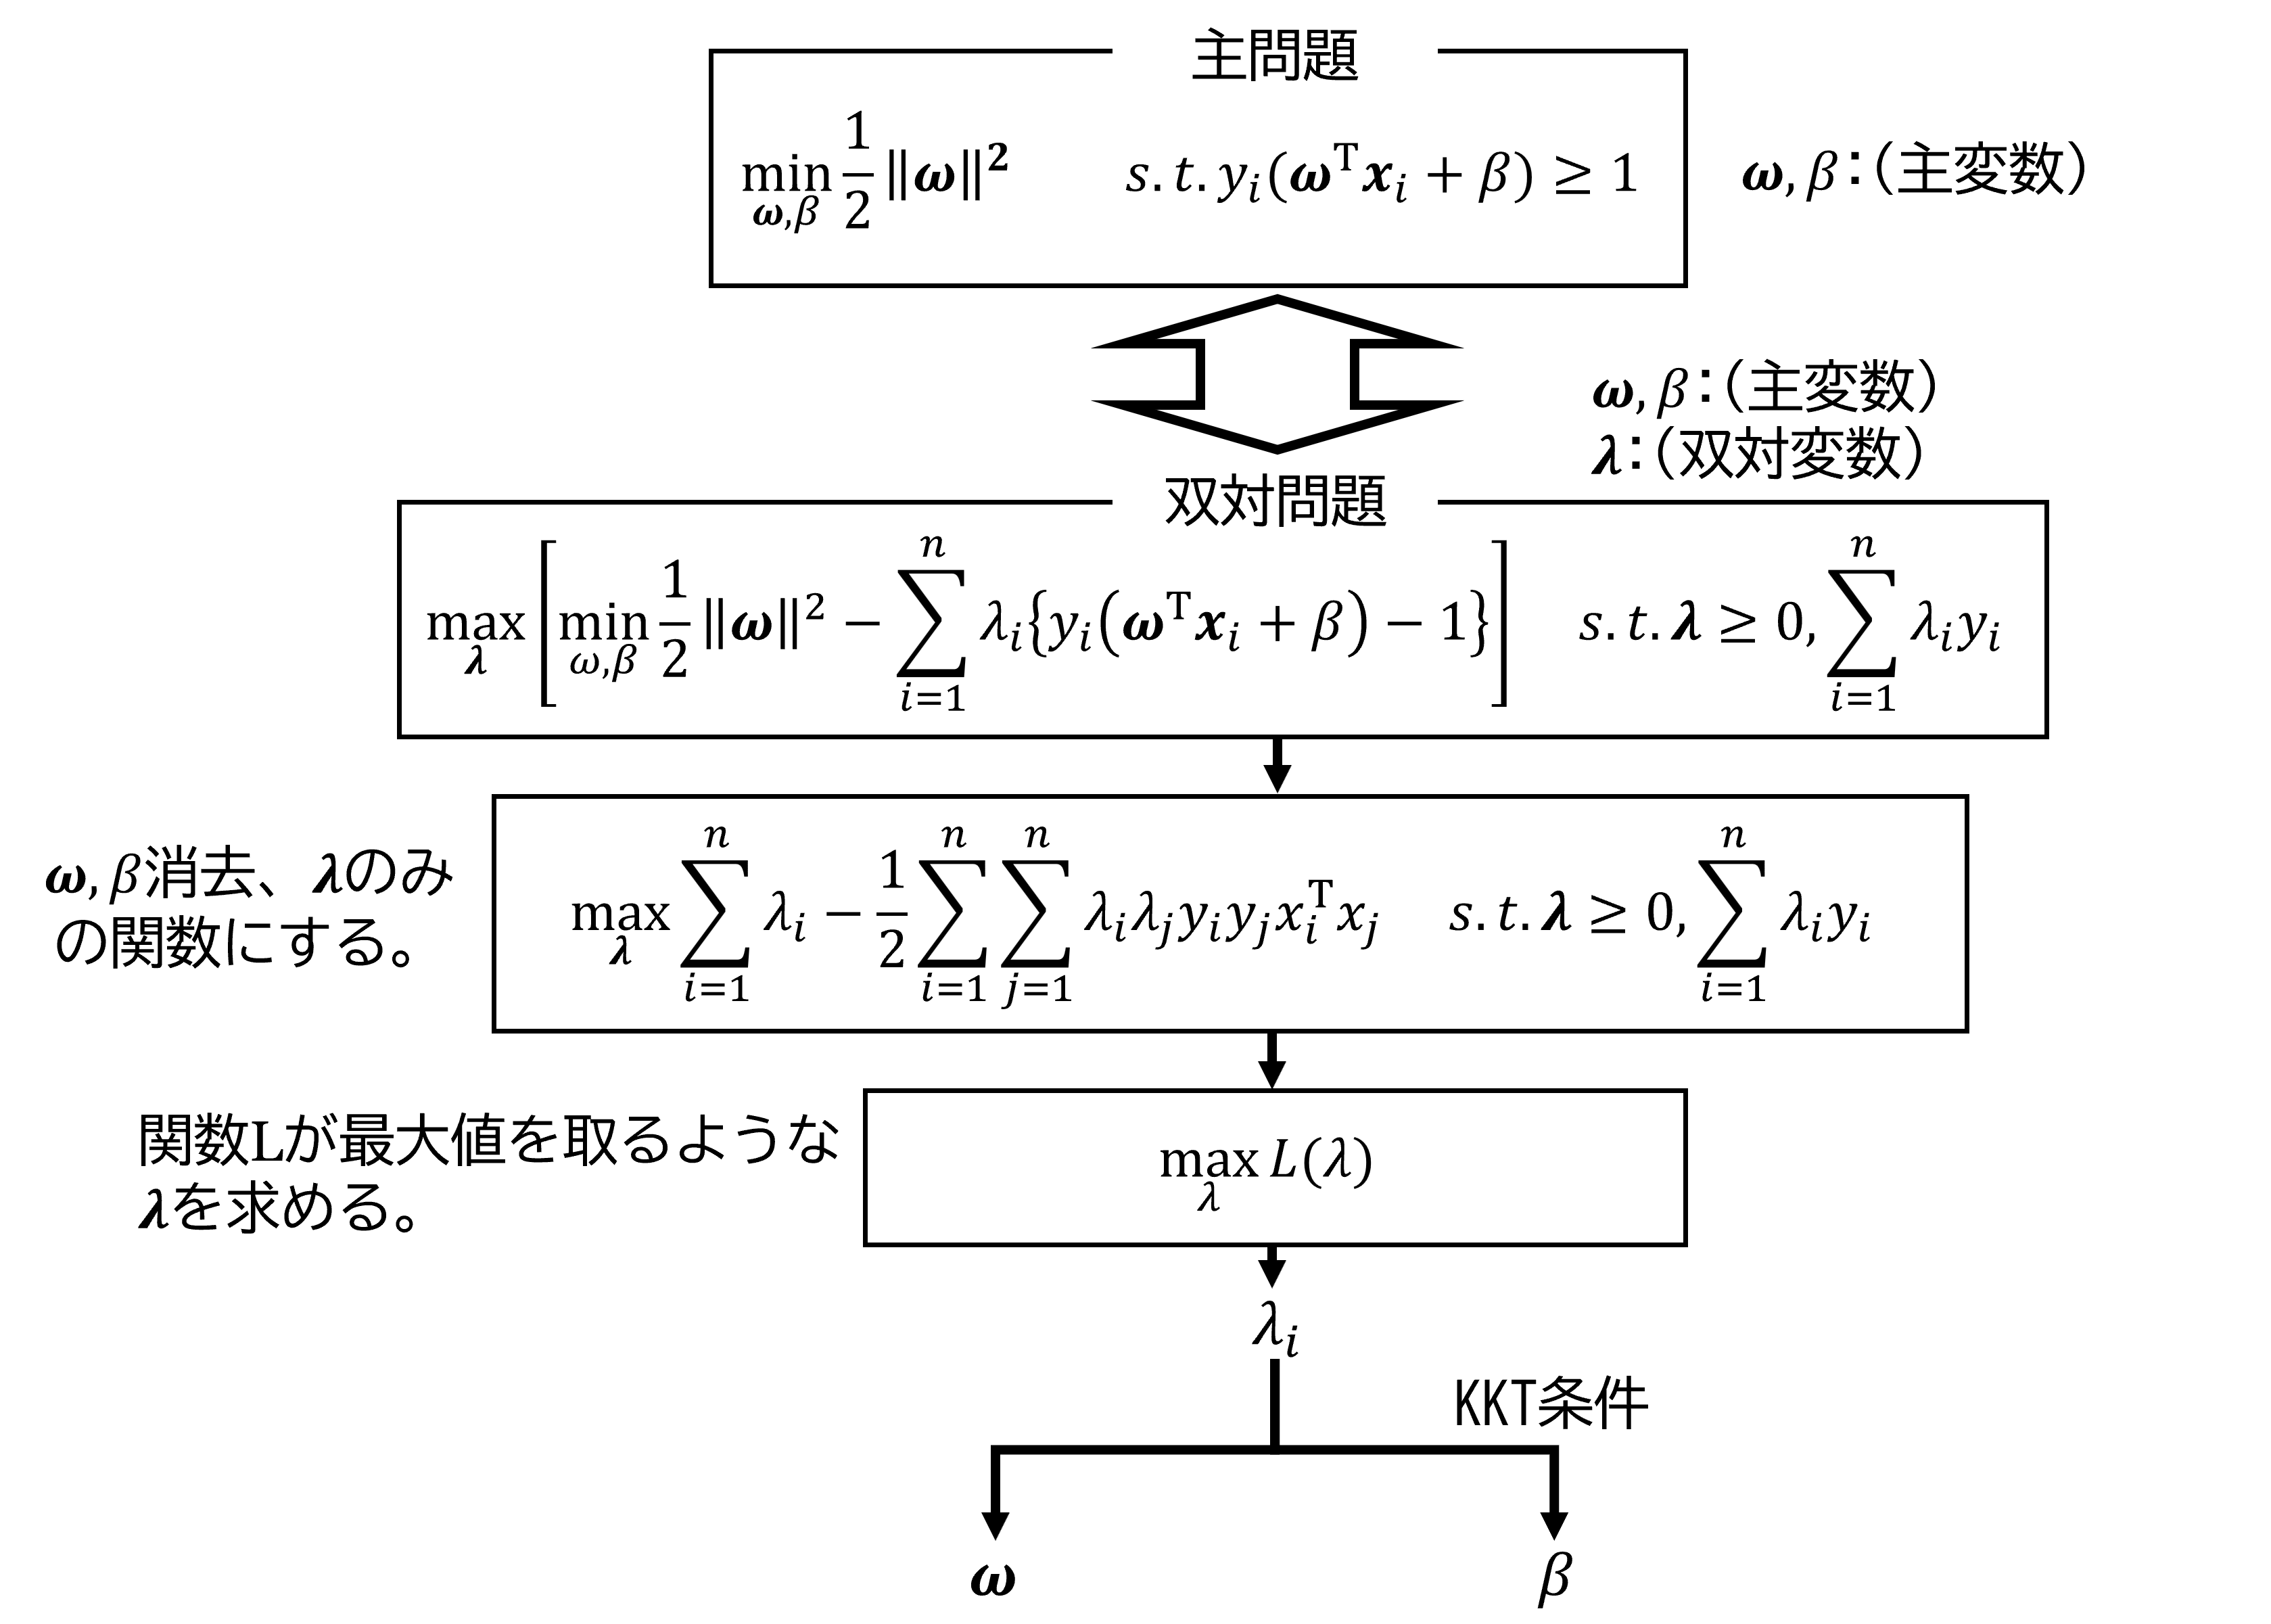
\includegraphics[width=0.8\textwidth]{image/svmmatome.png}
    \caption{SVMの流れ}
    \label{flow}
\end{figure}
カーネル関数を用いた線形SVMの導出方法をまとめる.
求める分類境界の式は式(\ref{nonlinbord2})で表され,パラメータ$\bm{\omega},\beta$を最適化する必要がある.
\begin{equation}
    \label{nonlinbord2}
    f(\bm{x}) = \bm{\omega}^\mathsf{T}\phi(\bm{x}) + \beta
\end{equation}

$\bm{\omega},\beta$を最適化するために式(\ref{nonlinhardmargin})の最適化問題を解く.
\begin{equation}
    \label{nonlinhardmargin}
    \begin{gathered}
        \min_{\bm{\omega},\beta}\frac{1}{2}\begin{Vmatrix}\bm{\omega}\end{Vmatrix}^2\\
        \text{s.t. } y_i(\bm{\omega}^\mathsf{T}\phi(\bm{x}_i) + \beta) \geq 1 \quad (i=1,2\dots n) 
    \end{gathered}
\end{equation}
$\bm{\omega}$についての主問題を解くのは困難であるため$\bm{\lambda}$についての双対問題である式(\ref{nonlindual})を考える.
\begin{equation}
    \begin{gathered}
        \max_{\bm{\lambda}}\left(\sum_{i=1}^{n}\lambda_i-\frac{1}{2}\sum_{i=1}^{n}\sum_{j=1}^{n}\lambda_i\lambda_jy_iy_jK(\bm{x}_i,\bm{x}_j)\right)\\
        \text{s.t. }\sum_{i=1}^{n}\lambda_iy_i=0,0\leq\lambda_i\leq C \tag{\ref{nonlinkarnel}}
    \end{gathered}
\end{equation}
この$\bm{\lambda}$についての双対問題を解き$\bm{\lambda}$を式(\ref{nonlinbeta})に代入することで,
分類境界を決定するパラメータ$\beta$が得られる.このときスパース性よりサポートベクトル以外の$\lambda_i$は考えなくてよい.
\begin{equation}
    \beta = \frac{1}{|SV|}\sum_{i \in SV}\left(y_i - \sum_{i \in SV}\lambda_jy_jK(\bm{x}_i,\bm{x}_j)\right) \tag{\ref{nonlinbeta}}
\end{equation}
また,分類境界の式は式(\ref{NewNonLinBordKarnel})のように書き換えられるため,
$\bm{\omega}$を求めることなく分類境界の式を求められる.
\begin{equation}
    f(\bm{x}) = \sum_{i \in SV}^{}\lambda_iy_iK(\bm{x},\bm{x}_i) + \beta \tag{\ref{NewNonLinBordKarnel}}
\end{equation}
得られた分類境界について,未知のデータに対してもスパース性により分類の計算に使う$\lambda_i$はサポートベクトルのもののみとなる.
%
%
\printbibliography

\end{document}
% \section{補足}
% KKT条件の章で取り上げた最適化問題(\ref{inequ})は以下の問題(\ref{syu})に変換される.
% \begin{equation}
%     \label{syu}
%     \underset{\bm{x}}{\min} \underset{\bm{\lambda} \geq 0,\bm{\mu}}{\max}L(\bm{x},\bm{\lambda},\bm{\mu})
% \end{equation}
% 変換された問題の双対問題は
% \begin{equation}
%     \label{dual}
%     \begin{gathered}
%         \underset{\bm{\lambda} \geq 0,\bm{\mu}}{\max} D(\bm{\lambda},\bm{\mu})\\
%         ただし\\
%         D(\bm{\lambda},\bm{\mu}) = \underset{\bm{x}}{\min}L(\bm{x},\bm{\lambda},\bm{\mu})\\
%     \end{gathered}
% \end{equation}
%SVMとは制約付き最適化問題を解くことで最適な分類境界を得るアルゴリズム,
%制約が等式の時はハードマージン,不等式の時はソフトマージンとなる.
%非線形データを扱う時はカーネル関数を使うことでSVMを可能にする.